\documentclass[a4paper,10pt,twocolumn]{jsarticle}
\usepackage{myjlababsstyle}
\begin{document}
\section{その他}
その他の事項として、本節では表の記述方法とぶち抜きの図について記載する。

\subsection{表の記述}
論文を記述する際にも指摘したが、表においては数値は右詰にしなければならない。
また、ラベル部は中央揃えとすることが多い。

そのような設定をしたものを、表~\ref{table:face_rec}に示す。

\begin{table}[b]
\centering
\vspace{2mm}
\caption{WHLACによる顔表情認識率}
\label{table:face_rec}
\vspace{3mm}
\small
\begin{tabular}{r|r|r|r} \hline
\multicolumn{1}{c|}{Data \#} & \multicolumn{1}{c|}{Ave.} & \multicolumn{1}{c|}{Max.} & \multicolumn{1}{c}{Min.} \\ \hline\hline
1 &  0.67 (N/A) & 0.91 (39) & 0.46(21) \\ \hline
2 & 0.37 (N/A) & 0.50 (38) & 0.09(10) \\ \hline
3 & 0.65 (N/A) & 0.87 (45) & 0.28(10) \\ \hline\hline
\multicolumn{1}{c|}{Total Ave.} & 0.56 & 0.76 & 0.27 \\ \hline
\end{tabular}
\end{table} %

\subsection{二段ぶち抜きの図}
二段組の省略ではあるが、図表の設定(開始タグと終了タグを共に)を~\verb+figure*+ とすることで、左右の段をぶち抜いて図表を入れることができる。
例を図\ref{fig:mp2}に示す。

\begin{screen}
{\small
\begin{verbatim}
\begin{figure*}[bt]
\centering
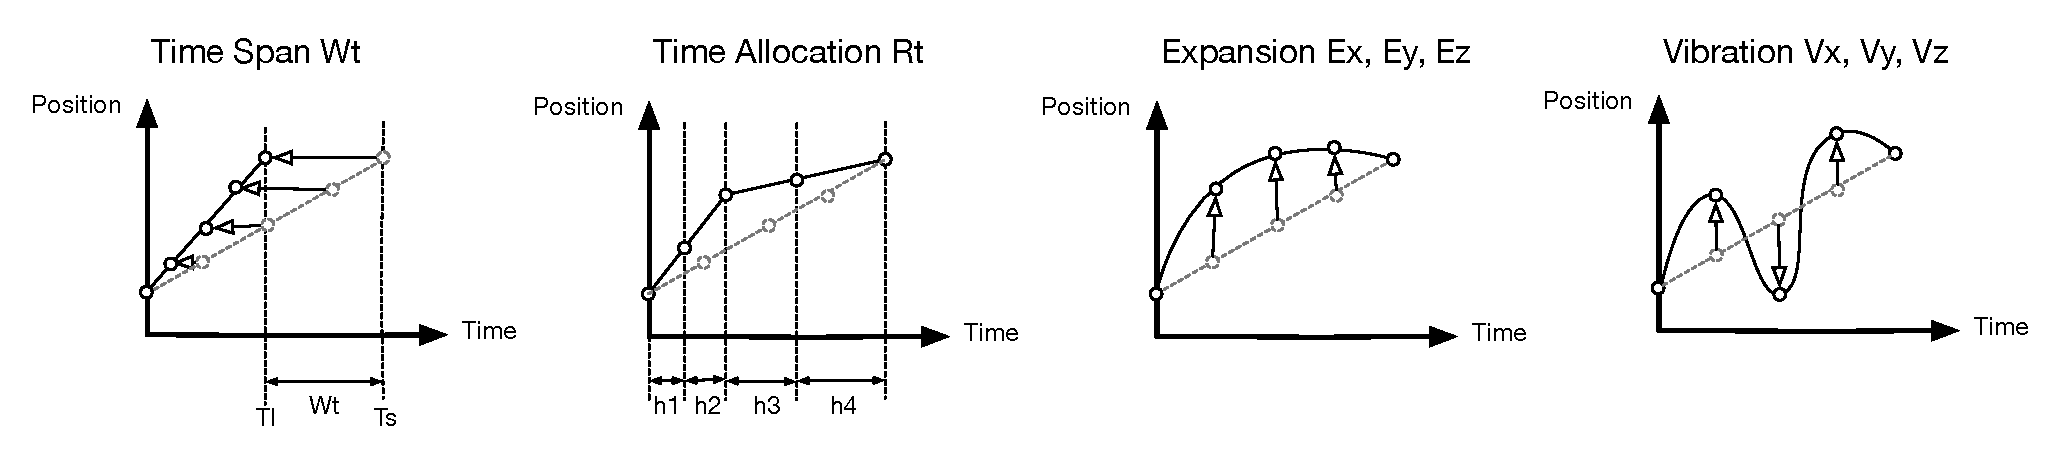
\includegraphics[width=14cm]{mp2.pdf}
\vspace{-7mm}
\caption{MMSの内部構成}
\label{fig:mp2}
\vspace{5mm}
\end{figure*}
\end{verbatim}
}
\end{screen}

\begin{figure*}[bt]
    \centering
    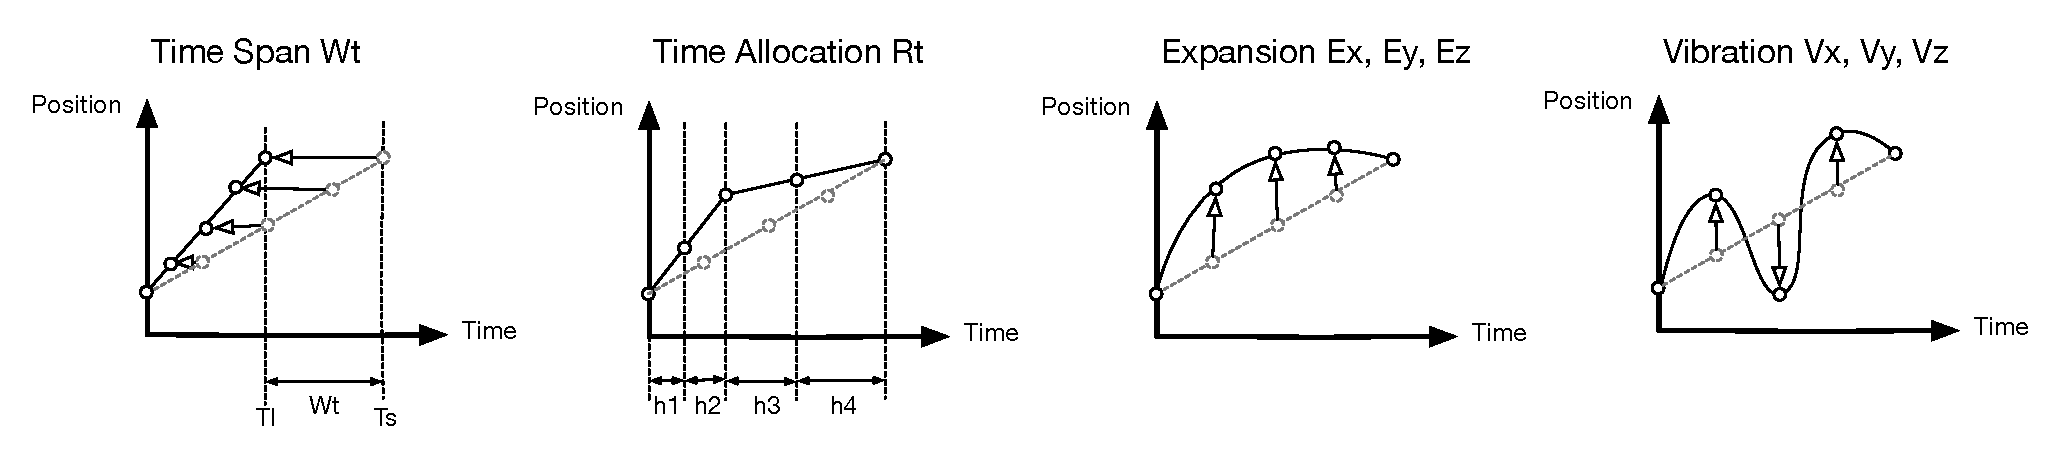
\includegraphics[width=18cm]{mp2.pdf}
    \vspace{-7mm}
    \caption{MMSの内部構成}
    \label{fig:mp2}
    \vspace{5mm}
\end{figure*}



%
\end{document}